\chapter{SW implementering og test }

\section{Implementering}
Softwaren i blodtryksmåleren er opbygget omkring 3-lags modellen. 

\begin{figure}[H]
	\centering
	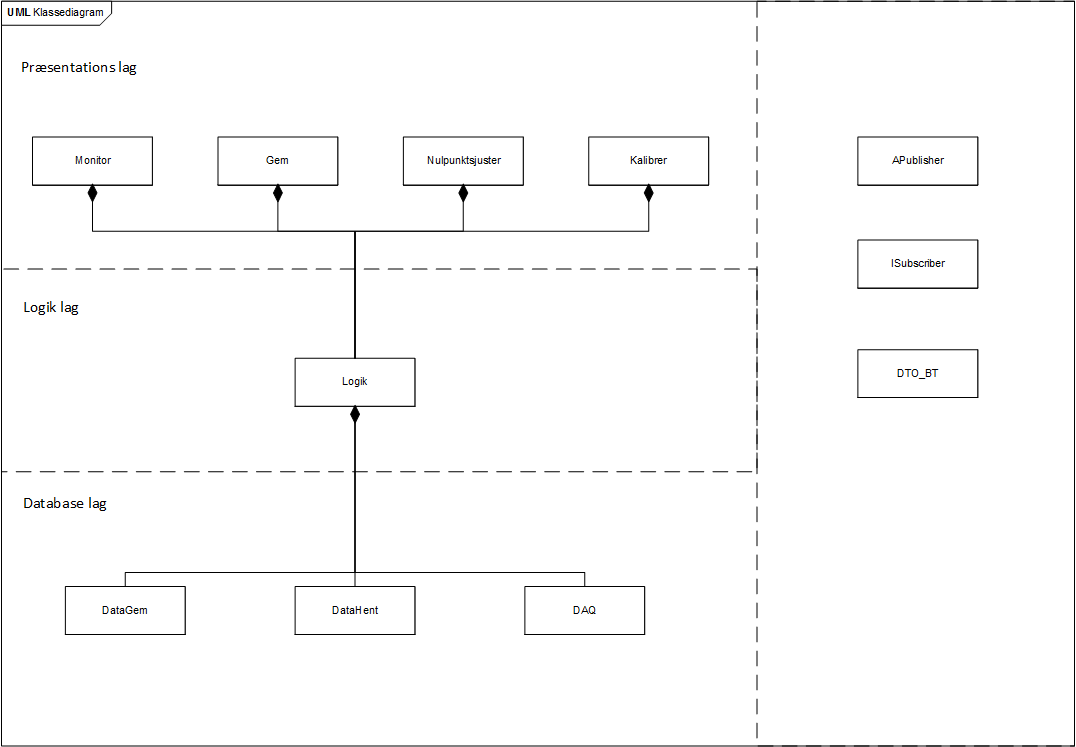
\includegraphics[width=1\textwidth]{Figurer/3lagsmodel_software}
	\caption{UML kompositions klassediagram}
\end{figure}

\begin{figure}[H]
	\centering
	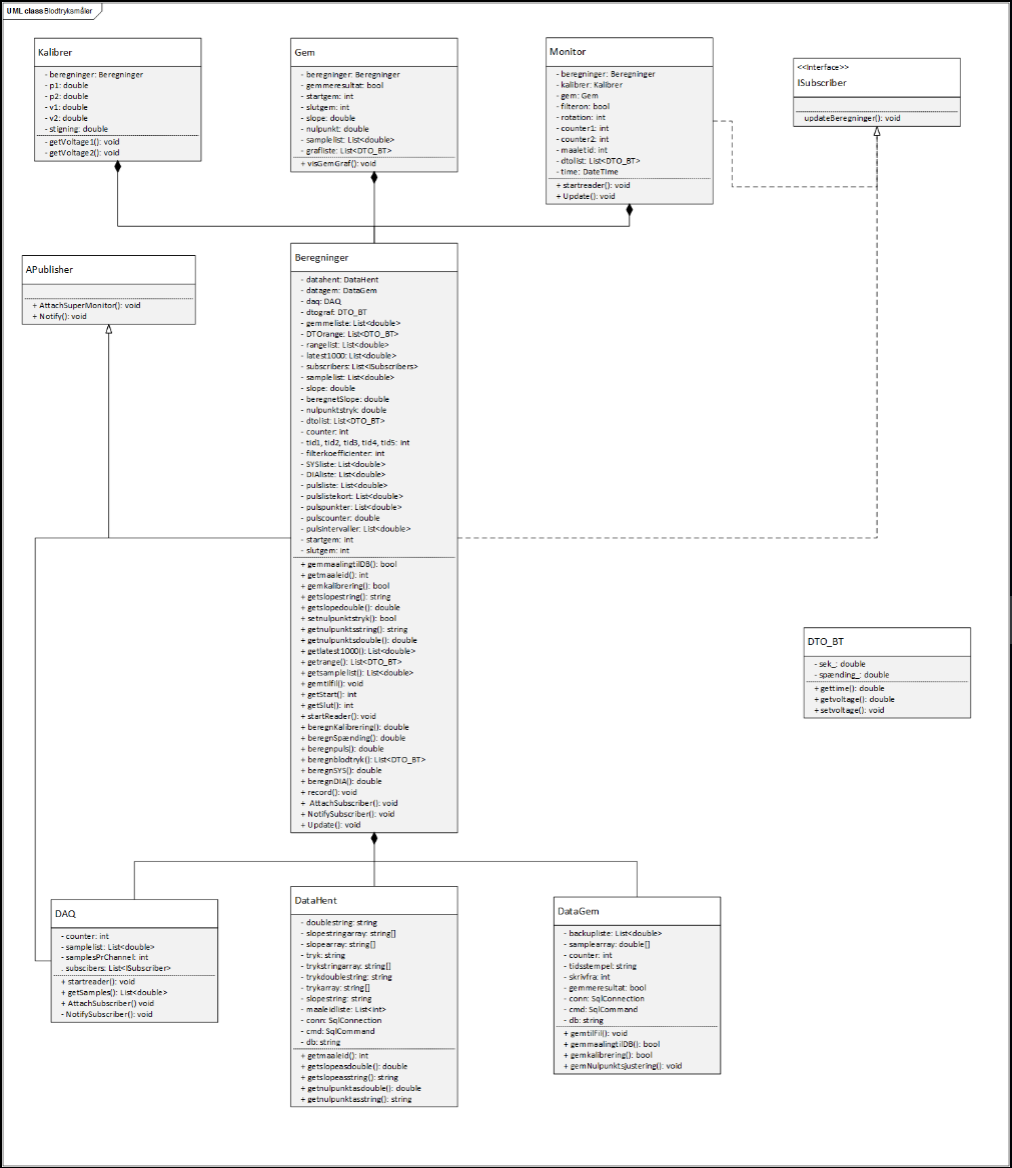
\includegraphics[width=1\textwidth]{Figurer/classdiagram}
	\caption{Klassediagram}
\end{figure}

\subsection{Datalag}
Datalaget kommunikerer med DAQ, database og computers HDD. 

\subsubsection{DAQ}
Herunder er en klasse, DAQ, hovedsageligt med software fra National Instruments, der kan udveksle data med den fysiske DAQ 6009. Denne kan betragtes som af typen ”black box”. Dette betyder at undertegnede ikke har et begreb om den interne mekanisme i klassen. Som udgangspunkt ved vi at funktionen af klassen er at levere data omkring de målinger der foretages i den fysiske DAQ.\\
De styrbare parametre i denne klasse er bl.a.: Sampling frekvens og måleområde. 

\subsubsection{Datahent}
Klassen henter data fra database og lokale tekstfiler. Fra databasen indhentes data om tidligere målingers nummerering således at de målinger der skal gemmes i fremtiden kan blive nummereret korrekt.\\
De lokale tekstfiler indeholder data omkring tidligere kalibreringer og nulpunktsjusteringer.

\subsubsection{DataGem}
Klassen gemmer data, på database, og lokale tekstfiler.

\subsection{Logik lag}

\subsubsection{Beregninger}
Beregninger er hovedsageligt et lag hvor logiske beregninger foretages.\\
Herunder beregnes ting som systolisk og diastolisk blodtryk og puls. Beregninger i forbindelse med kalibrering og nulpunktsjustering foregår også her. Ydermere forbinder logik laget data laget med form laget. Dette tillader at metoder fra datalaget kan anvendes fra form laget.

\subsection{Præsentations lag}
\begin{figure}[H]
	\centering
	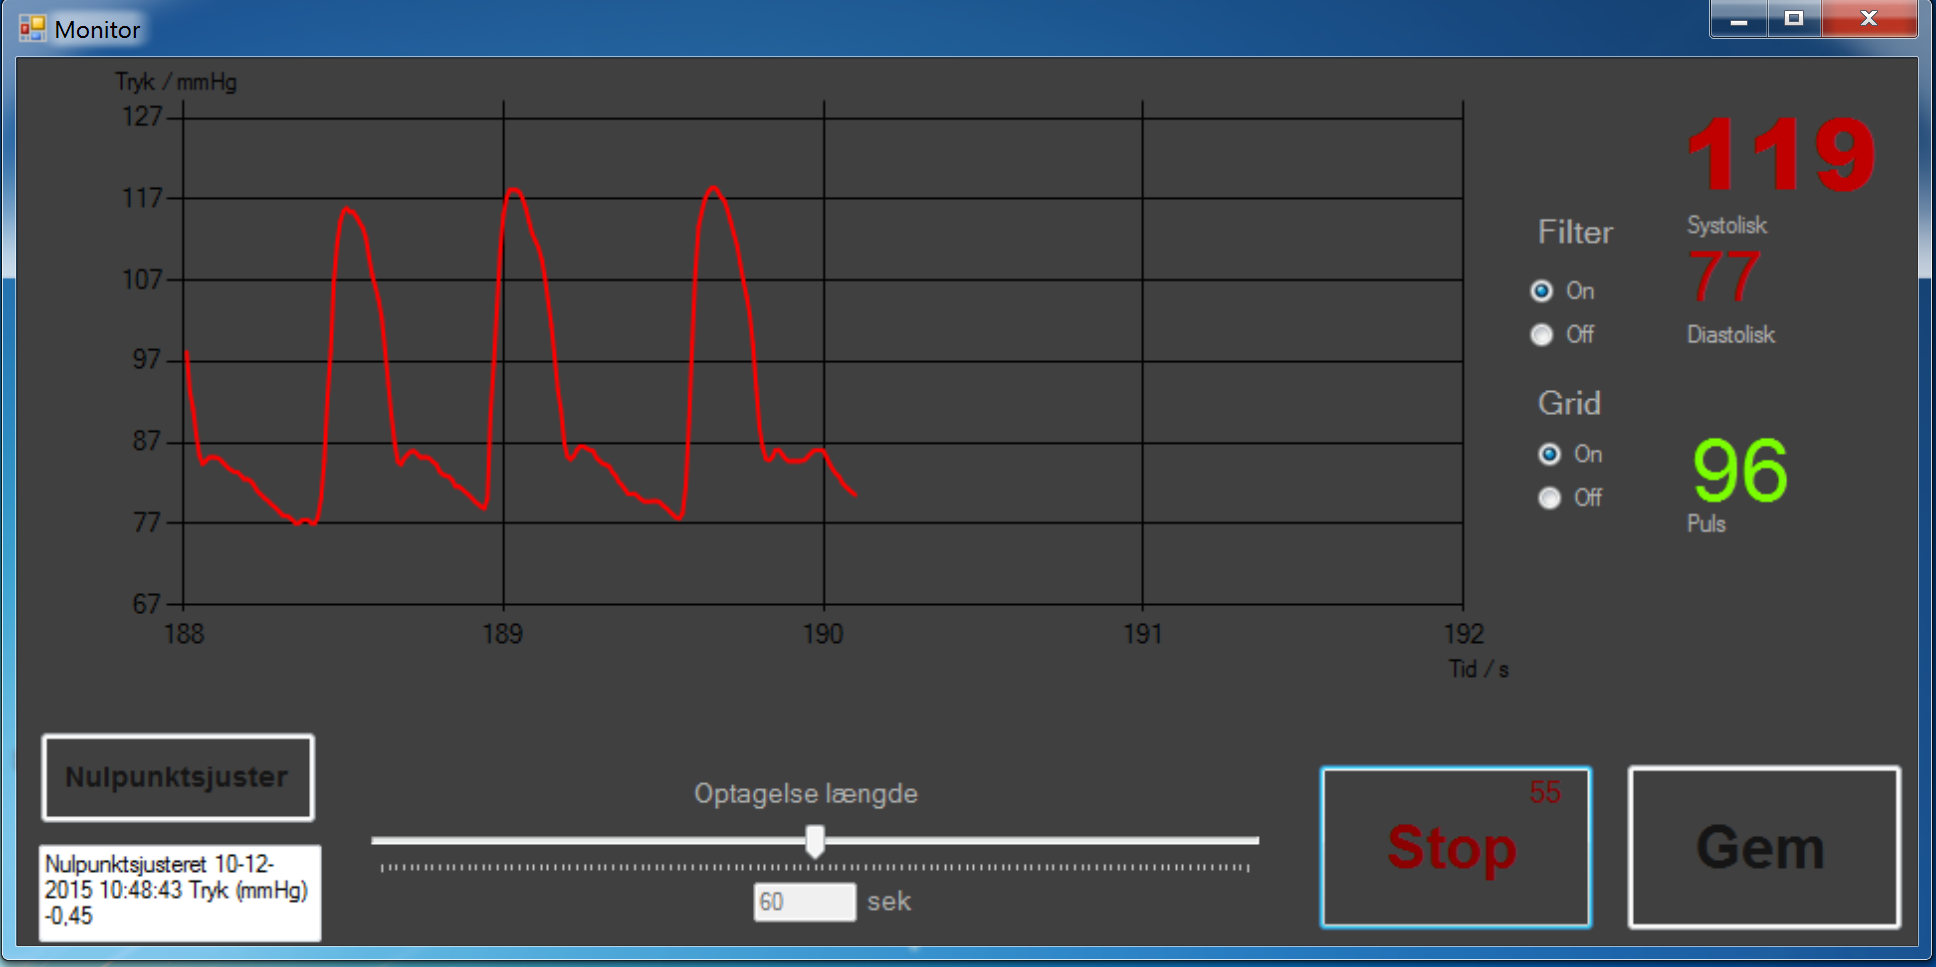
\includegraphics[width=1\textwidth]{Figurer/Monitor_vindue_Recording}
	\caption{Monitor med igangsat måling}
\end{figure}

\subsubsection{Monitor}
Monitorlaget er brugerens generelle visuelle interaktionslag med systemet. Heri observeres udskrevne blodtrykssignaler over 4-sekunders intervaller. Værdierne puls, systolisk og diastolisk blodtryk udskrives også her. Designet er inspireret fra i forvejen eksisterende blodtryks monitoreringssystemer. \\
Der er mulighed for at vælge en længde af optagelse af måling, op påbegyndelse/stoppe med en ”Rec” knap. Herefter kan gem vinduet åbnes hvor den optagne sekvens kan gemmes. Der er en knap til udførelse af nulpunktsjustering. Den kørende måling kan vises med et filter, eller uden med 2 radio butons. Y- og X-akse kan påsættes med 2 radio buttons. 

\subsubsection{Gem}
Vinduet udskriver den optagne sekvens i et vindue der visuelt ligner monitor vinduet. Der er to tekstbokse, hvor en kommentar og et navn, for den ansvarlige af målingen, kan indtastes.

\subsubsection{Kalibrer}
Vinduet indeholder to tekstbokse til indtastning af tryk og tekstbokse til dertilhørende spænding. Spændingerne kan måles automatisk ved tryk på knapperne ”mål”.
Kalibreringskonstanten kan udregnes med knappen ”Beregn”, og gemmes og anvendes ved tryk på ”OK” knappen.

\subsection{DTO}
DTO er et namespace det indeholder data transfer object (DTO). Alle den andre lag ”kender” dette lag, og kan oprette instanser af klassen DTO.\\
Denne klasse har attributterne tid og spænding. Formålet med denne klasse er at overføre sampleværdier fra DAQ i et format der har en korrekt tidsværdi, samt et tryk (blodtryk) korrigeret for nulpunktstryk samt kalibrering.

\subsubsection{Publisher/subscriber pattern}
Data ”strømmen” fra DAQ klassen, er styrende for alle de andre klasser, bl.a. udskrivning af blodtrykket i monitor vinduet. Den fysiske DAQ måler i med 1000 Hz og returnerer data til DAQ klassen med 50 ms intervaller. Dette måleinterval indeholder 50 sampleværdier. Disse data sendes videre til beregninger klassen, og fra beregninger klassen til monitor klassen vha. Publisher/Subscriber mønstret. Når data befinder sig i monitor klassen kan der laver logiske beregninger og manipulation på data i beregninger klassen.
Forholdet imellem klasserne er således; DAQ klassen og beregninger klassen har et publisher/subscriber forhold, og  beregninger og monitor har et publisher/subscriber forhold.

\subsection{Metodebeskrivelser}
Metoden der beregner puls, har to logiske grene til udregning af pulsen. Den første (til venstre i diagram) regner pulsen når der er mellem 3000 og 10000 samples til rådighed, altså når den fysiske DAQ har målt imellem 3 og 10 sekunder.\\
Metodikken består i at lokalisere toppunkter i signalet, for at udregne det gennemsnitlige interval herimellem. Herudfra kan pulsen estimeres. \\
En for-løkke bruges til at evaluere alle sampleværdier i forhold til de før liggende og efterfølgende samples. Hvis værdien på den pågældende sample har større værdi end den før liggende og efterfølgende, gemmes tidspunktet for dette sample i en liste.\\ 
For at sikre at ”toppunktet” ikke er et mindre toppunkt, fra fx støj eller højfrekvent signalindhold, evalueres der kun for hver 50'ende værdier, og tidspunktet gemmes kun hvis værdien ligger 0,1 V over gennemsnittet af alle sampleværdier der evalueres. Ud fra gennemsnitsintervallet imellem toppunkterne beregnes pulsen.
\\
\\
Den anden logiske gren regner pulsen når der er over 10000 samples til rådighed, altså efter den fysiske DAQ har målt i over 10 sekunder.\\ 
Metodikken er den samme som ovenfor, men i stedet for at gemme et tidspunkt for toppunktet, tælles en counter op. Når antallet af toppunkter for 10 sekunder er fundet, kan pulsen beregnes.

\begin{figure}[H]
	\centering
	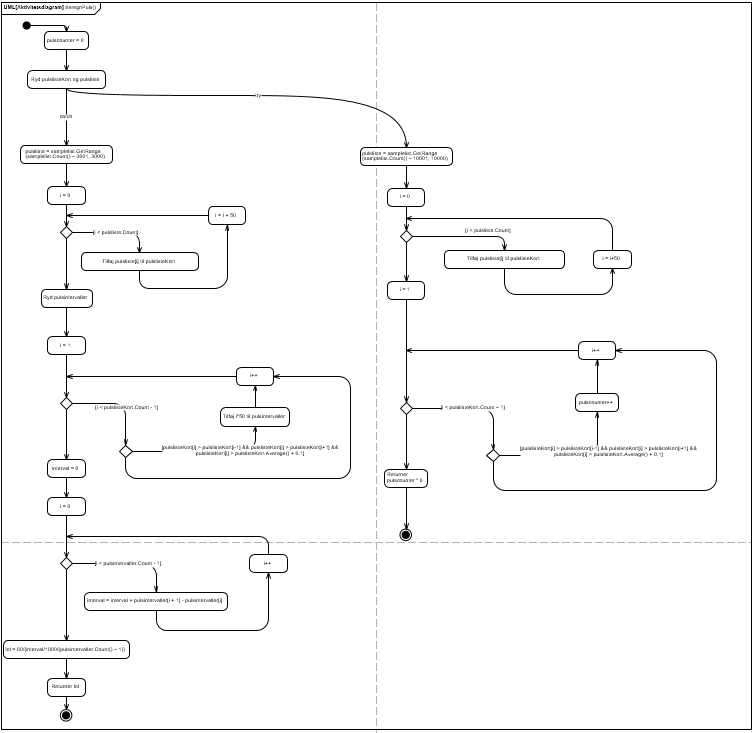
\includegraphics[width=1\textwidth]{Figurer/aktivitetsdiagram_beregnPuls}
	\caption{Aktivitetsdiagram over beregnpuls}
\end{figure}


\subsection{Sekvensdiagrammer}
******INDSÆT KORT INDLEDNING TIL NEDENSTÅENDE SEKVENSDIAGRAMMER******

\begin{figure}[H]
	\centering
	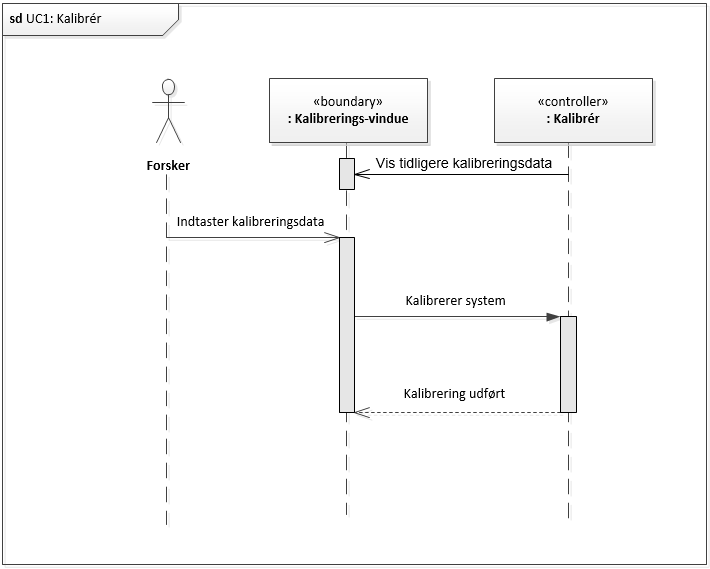
\includegraphics[width=1\textwidth]{Figurer/UC1_SD}
	\caption{Sekvensdiagram for UC1}
\end{figure}

\begin{figure}[H]
	\centering
	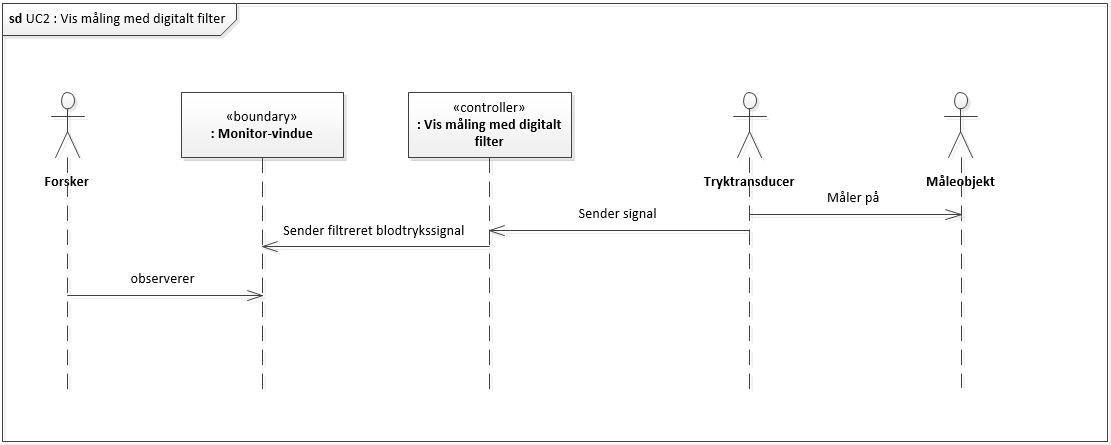
\includegraphics[width=1\textwidth]{Figurer/UC2_SD}
	\caption{Sekvensdiagram for UC2}
\end{figure}

\begin{figure}[H]
	\centering
	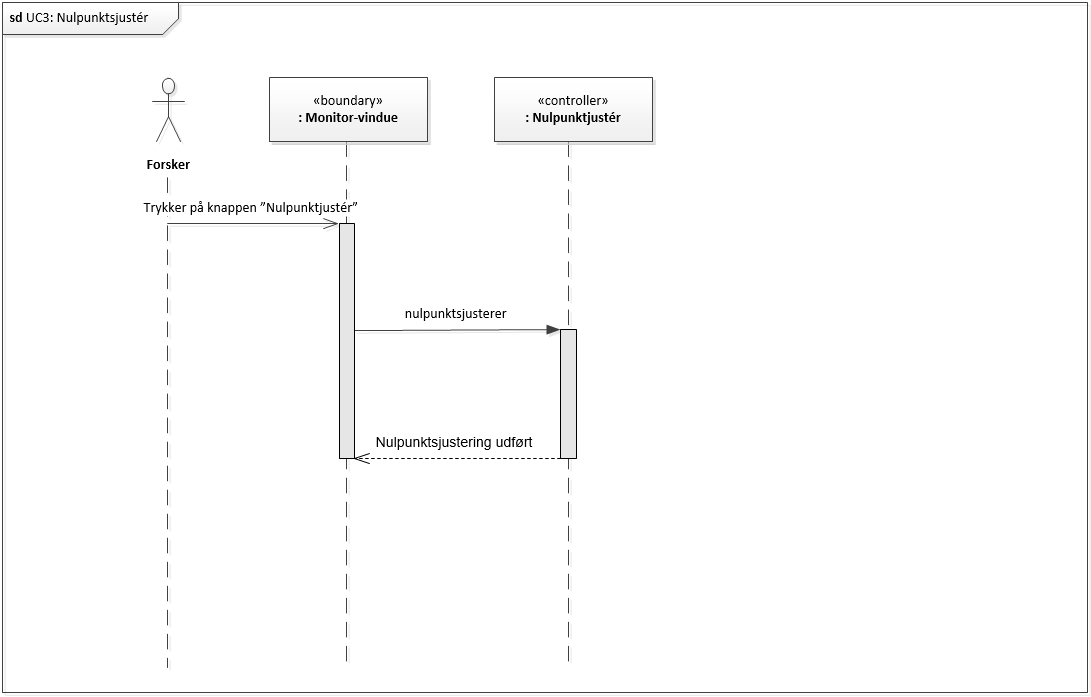
\includegraphics[width=1\textwidth]{Figurer/UC3_SD}
	\caption{Sekvensdiagram for UC3}
\end{figure}

\begin{figure}[H]
	\centering
	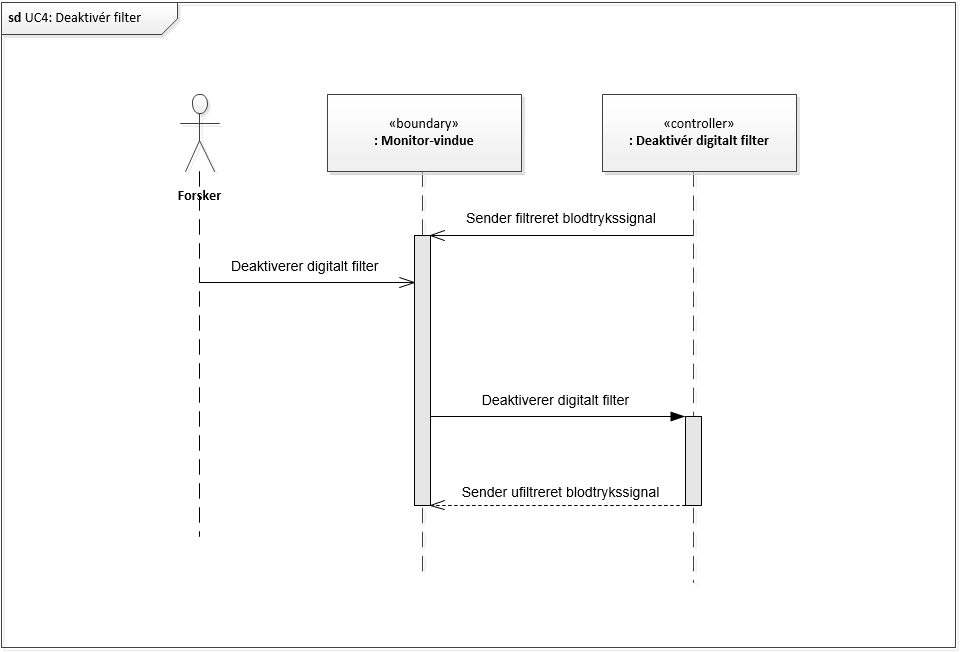
\includegraphics[width=1\textwidth]{Figurer/UC4_SD}
	\caption{Sekvensdiagram for UC4}
\end{figure}

\begin{figure}[H]
	\centering
	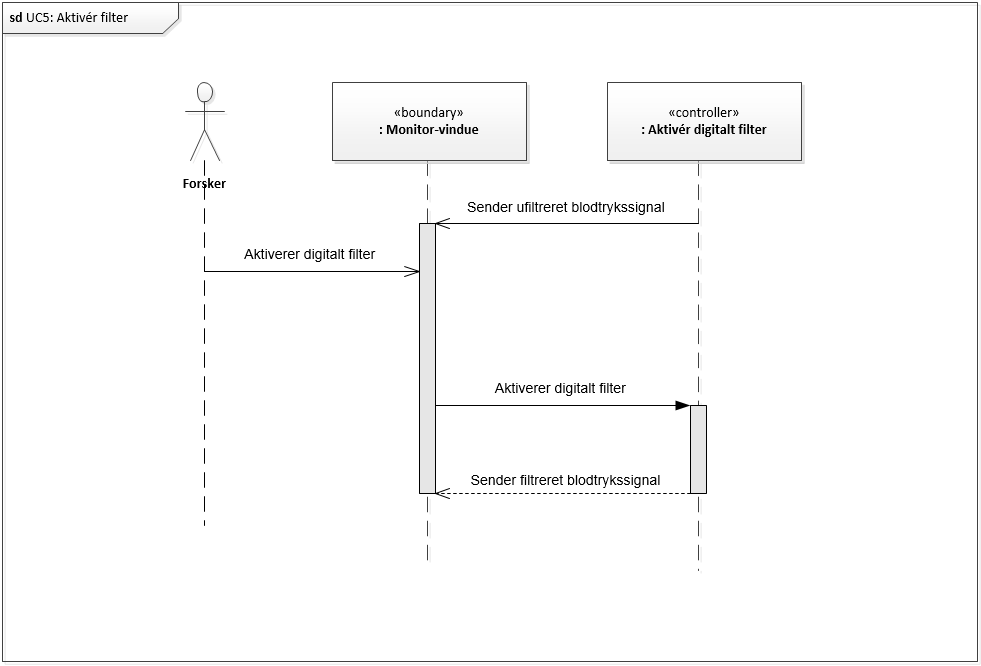
\includegraphics[width=1\textwidth]{Figurer/UC5_SD}
	\caption{Sekvensdiagram for UC5}
\end{figure}

\begin{figure}[H]
	\centering
	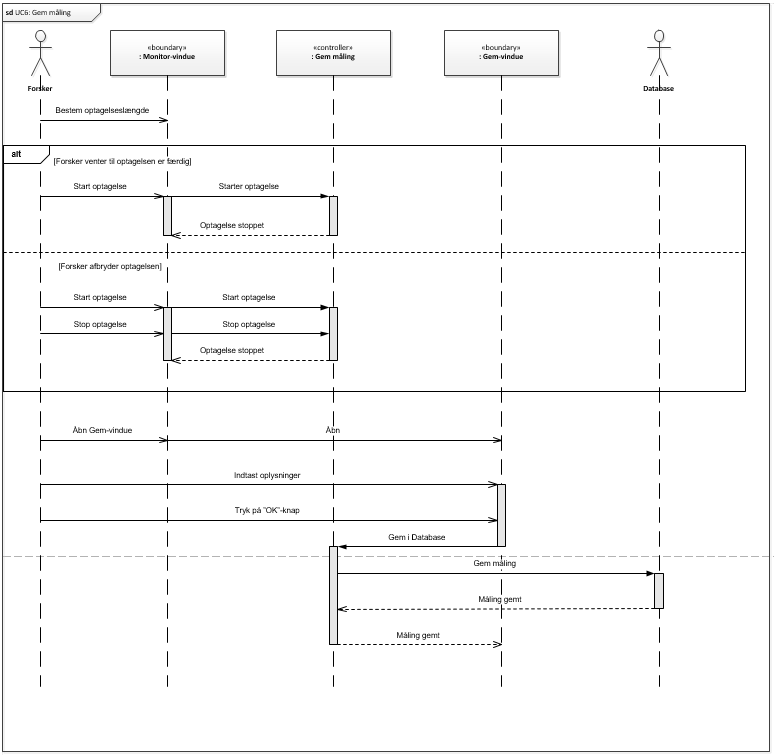
\includegraphics[width=1\textwidth]{Figurer/UC6_SD}
	\caption{Sekvensdiagram for UC6}
\end{figure}
